\documentclass[a4paper,11pt]{report}
\usepackage[T1]{fontenc}
\usepackage[utf8]{inputenc}
\usepackage{lmodern}
\usepackage[spanish]{babel}
\usepackage{graphicx}
\usepackage[top=3cm, bottom=2.5cm, inner=1.5cm, outer=2.5cm]{geometry} % Márgenes personalizados
\usepackage{float} % Permite posicionar mejor las figuras y tablas
\usepackage{amsmath} % Comandos para la escritura de fórmulas matemáticas de mayor complejidad
\usepackage{amsfonts} % Proporciona fuentes matemáticas
\usepackage{amssymb} % Proporciona símbolos matemáticos de la American Mathematical Society

\title{Digit Recognizer. \\ 
  Classify handwritten digits using the famous MNIST data.\\
  Organizacion de Datos 75.06}
\author{Joaquín Blanco. Padrón 94653.\\
  Ruben Alvarado. Padrón.\\
  Diego Ripetour. Padrón.\\
  Grupo en Kaggle: The Thompsons}

\begin{document}

\maketitle
\tableofcontents

\begin{abstract}
En este informe se presentara el diseño elegido para realizar el reconocimiento de dígitos manuscritos. Nuestra propuesta comprende una combinación de algoritmos de clasificación simples, los cuales fueron testeados de forma independiente de tal manera que se puedan determinar aportes y limitaciones.
\end{abstract}
%include == include en c
%Es preferible que cada cual tenga que trabajar en su parte
%Sin tener que lidiar con el resto. A menos que así lo quiera
\chapter{Análisis Inicial de los datos.}
Previamente al diseño de la solución, se decidió realizar un análisis de los datos de entrenamiento tal que se pueda determinar sus características y formas en que las pueden ser aprovechadas.

En principio podemos decir que contamos con 42000 imágenes de 28 píxeles de ancho por 28 píxeles de alto. Cada una esta ligada a una clase de entre 10 que pueden ser 0,1,...,9. 

En la Tabla 1.1 se puede observar el porcentaje de imágenes de cada una de las clases que existen en el set de entrenamiento y como bien se puede observar, ser puede decir que el mismo esta balanceado. 

\begin{table}[htp]
  \caption{Porcentaje de imágenes de cada una de las clases en el train}
  \label{porc}

  \begin{center}
    \begin{tabular}{|c|c|c|c|c|c|c|c|c|c|c|}
    \hline
      Clase&0&1&2&3&4&5&6&7&8&9 \\
    \hline
      Porcentaje&9.83&11.15&9.94&10.35&9.69&9.03&9.85&10.47&9.67&9.97 \\
    \hline
    \end{tabular}
  \end{center}
\end{table}

Por otro lado si realizamos un promedio de todas las imágenes y observamos los valores obtenidos, daremos cuenta de que existen pixels cuyo valor es 0. Esto nos da pie para pensar que podríamos a llegar a prescindir de algunos atributos, reduciendo así el costo computacional que requerirá procesar todos estos datos. Mas adelante en el informe veremos que esto efectivamente es así.
\begin{figure}[htp]
  \begin{center}
    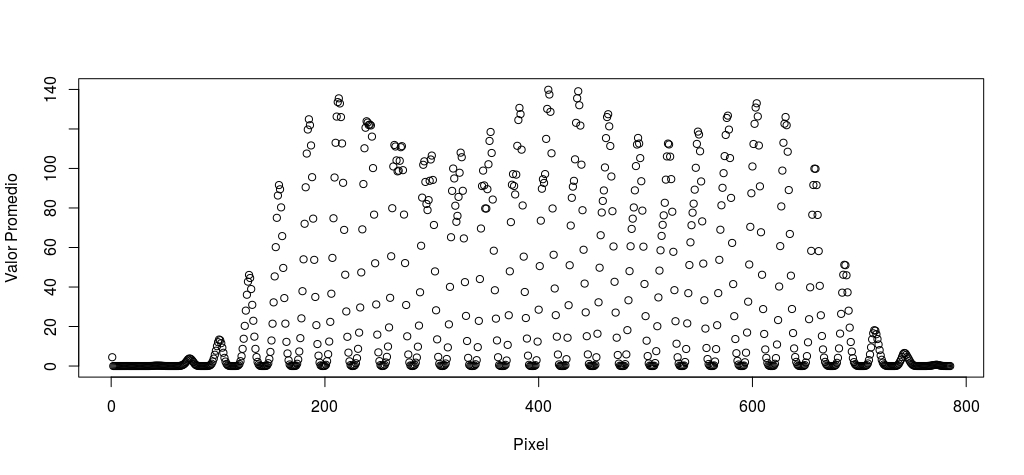
\includegraphics[width=15cm]{promImg.jpeg}
    \caption{Valores promedio de cada pixel}
    \label{promPix}
  \end{center}
\end{figure}


\end{document}
